\section{Evaluation}
\label{section:evaluation}
In the following chapter the mobile implication of \gls{see} will be evaluated in a user study.
Therefore, the mobile application will be compared with the desktop version.

This chapter will start with a description of the desktop version and its main differences in section \ref{desktop}.
Continuing with a defined aim and the precise hypotheses for the user study in section \ref{aim}.
After sketching the first experiment set up in section \ref{experiment} the actual experiment set up will be discussed in detail in section \ref{real} including the used survey tool, questionnaires and the pilot study.
\subsection{SEE Desktop}
\label{desktop}
In this section the desktop version of \gls{see} will be explained.
In this evaluation the mobile version of \gls{see} will be compared with the desktop version.
Therefore, it is necessary to take a deeper look at the differences between those two versions.
Especially at how the interactions differ and what impact it could have on the user experience.

One outstanding difference from the desktop version to the mobile version is the selection of the interaction modes.
While in the mobile version the menu for the interaction modes is always visible in the desktop version by pressing space a menu screen opens as seen in figure \ref{fig:menu}.
Alternatively interaction modes can be changed by pressing one of the "1-9" keys, which, however requires the user to memorize which number belongs to which mode.

\begin{figure}[htb]
  \centering
  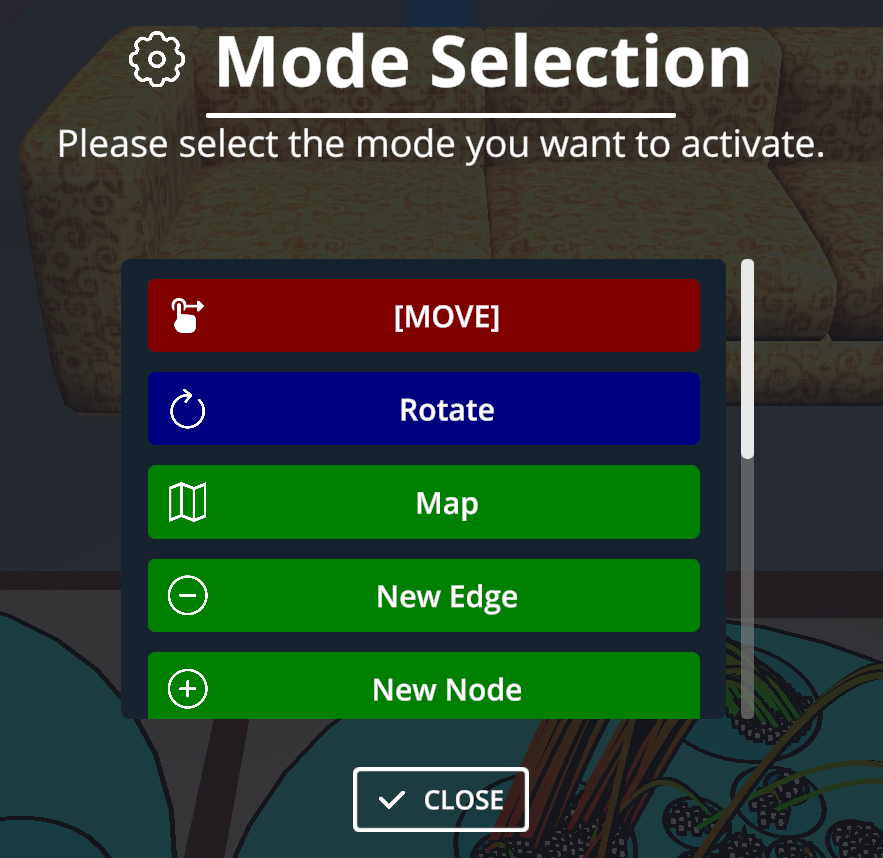
\includegraphics[width=0.8\textwidth]{Evaluation/img/menu.png}
  \caption{The desktop menu for selecting interaction modes.}\label{fig:menu}
\end{figure}

Another difference is the type of user input.
The desktop version uses mouse hovering to display the name of a hovered \gls{node} or \gls{plane}.
This is a faster method then touching the object first in the mobile version.
In addition to that in the mobile version the object also has to be deselected otherwise there will be a lot of \gls{node} and \gls{plane} names displayed, and it will soon get quite messy.
Also, the precision of object selection differs because touch input can never be as precise as selecting with a mouse cursor.
This could force the mobile user to zoom further in because with a touch input it will not be possible to select small objects like it might be with a cursor.
Which, of course, would require more time.

One more key difference is the available keyboard for desktop users.
It allows using \glspl{shortcut}, which makes some menu items unnecessary but also requires the user to memorize those \glspl{shortcut}.
The desktop version for example uses the "R" key in the move and rotation mode to recenter or rerotate a \gls{city}.
In the mobile version on the other side the user will find a button for both actions.
With the right amount of training both actions should probably equal in the amount of time they need but the mobile version sacrifices screen space for those buttons.
If however the user has to type more text like in renaming objects, the common desktop keyboard should come in handy as a study from \cite{kim2014differences} shows that even at a same keyboard size, a virtual one will lack in productivity.
\subsection{Aim and hypothesis}
\label{aim}
The aim of this user study is to answer the research question discussed in section \ref{research}.
In order of answering the research question the finished prototype of the mobile extension shall be evaluated.
Therefore, the system shall be compared on Android smartphones as well as desktop computers.
Comparing these two use cases shall give insight on how much impact the constraints of mobile devices have on the usability and overall user experience.
To measure the difference between the desktop and the mobile version the following hypotheses will be used.
The two aspects performance and usability will be measured in the following study and each aspect will have a null hypothesis and an alternative hypothesis.
\begin{enumerate}[{label=\alph*)}]
  \item \textbf{Performance:} The time required for a task in \gls{see} desktop will be called $t_D$ and for mobile $t_M$.
        \begin{itemize}
          \item \textit{Null Hypothesis} $H_{a0}$: The time required in \gls{see} mobile is higher or the same as the time required in \gls{see} desktop: $t_M \geq t_D$
          \item \textit{Alternative Hypothesis} $H_{a1}$: The time required in {\gls{see}} mobile is lower as the time required in \gls{see} desktop: $t_M < t_D$
        \end{itemize}
  \item \textbf{Usability:} Two aspects are measured for \gls{usability}. First the \gls{ASQ}-Score as a \gls{post-task} result and second the \gls{sus}-Score as a \gls{post-study} result.
        \begin{enumerate}[label=\roman*)]
          \item \textbf{ASQ:} Once again the aspect has to be split into three child aspects, because the three questions of the \gls{ASQ} are independent:
                \begin{enumerate}[{label=\arabic*)}]
                  \item The \gls{ASQ}-Score for \textit{effort} for \gls{see} desktop is called $A_{eD}$ and for \gls{see} mobile is called $A_{eM}$
                        \begin{itemize}
                          \item \textit{Null Hypothesis} $H_{b0}$: The \gls{ASQ}-Score for \textit{effort} is higher or even for \gls{see} desktop than on \gls{see} mobile: $A_{eD} \geq A_{eM}$
                          \item \textit{Alternative Hypothesis} $H_{b1}$: The \gls{ASQ}-Score for \textit{effort} is lower for \gls{see} desktop than on \gls{see} mobile: $A_{eD} < A_{eM}$
                        \end{itemize}
                  \item The \gls{ASQ}-Score for \textit{complexity} for \gls{see} desktop is called $A_{cD}$ and for \gls{see} mobile is called $A_{cM}$
                        \begin{itemize}
                          \item \textit{Null Hypothesis} $H_{c0}$: The \gls{ASQ}-Score for \textit{complexity} is higher or even for \gls{see} desktop than on \gls{see} mobile: $A_{cD} \geq A_{cM}$
                          \item \textit{Alternative Hypothesis} $H_{c1}$: The \gls{ASQ}-Score for \textit{complexity} is lower for \gls{see} desktop than on \gls{see} mobile: $A_{cD} < A_{cM}$
                        \end{itemize}
                  \item The \gls{ASQ}-Score for \textit{information} for \gls{see} desktop is called $A_{iD}$ and for \gls{see} mobile is called $A_{iM}$
                        \begin{itemize}
                          \item \textit{Null Hypothesis} $H_{d0}$: The \gls{ASQ}-Score for \textit{information} is higher or even for \gls{see} desktop than on \gls{see} mobile: $A_{iD} \geq A_{iM}$
                          \item \textit{Alternative Hypothesis} $H_{d1}$: The \gls{ASQ}-Score for \textit{information} is lower for \gls{see} desktop than on \gls{see} mobile: $A_{iD} < A_{iM}$
                        \end{itemize}
                \end{enumerate}

          \item \textbf{SUS:} The \gls{sus}-Score is called $S_D$ for \gls{see} desktop and $S_M$ for \gls{see} mobile.
                \begin{itemize}
                  \item \textit{Null Hypothesis} $H_{e0}$: The \gls{sus}-Score is higher or even for \gls{see} desktop than for \gls{see} mobile: $S_D \geq S_M$
                  \item \textit{Alternative Hypothesis} $H_{e1}$: The \gls{sus}-Score is lower for \gls{see} desktop than for \gls{see} mobile: $S_D < S_M$
                \end{itemize}
        \end{enumerate}
\end{enumerate}

The experiment will be participated different groups:
\begin{enumerate}
  \item \textbf{\gls{see}-developer:} They are already experienced with \gls{see}-desktop.
        They are also experienced with software development and with first person games because they tried at least \gls{see} itself, which counts as first person game experience.
  \item \textbf{Non-\gls{see}-developer:} This group has to be divided into four subgroups as follows:
        \begin{itemize}
          \item \textbf{Software development and third person game experience:} They are more likely to understand the \gls{city} metaphor and are also more likely to be comfortable with the controls in \gls{see}.
          \item \textbf{Software development experience:} They are more likely to understand the \gls{city} metaphor and therefore might be able to find \glspl{node} faster.
          \item \textbf{First person game experience:} They are also more likely to be comfortable with the controls in \gls{see}.
          \item \textbf{No experience:} They do not benefit from experience and therefore have to learn the most to interact in \gls{see}
        \end{itemize}
\end{enumerate}

After the experiment the two versions of \gls{see} can be compared as well as all above listed groups. 
This should give a detailed answer to the research question of this thesis.
\subsection{Experiment set up}
\label{experiment}
The system shall be tested in two groups each starting with a different device.
Each group does the test on both devices, but one group will start with the mobile application and the other one with the desktop application.
The participants will be assigned random to the groups.
The testers will have various tasks to test the usability of the two applications.
Afterwards the users will get a survey in English to document their impressions.
\begin{figure}[H]
  \centering
  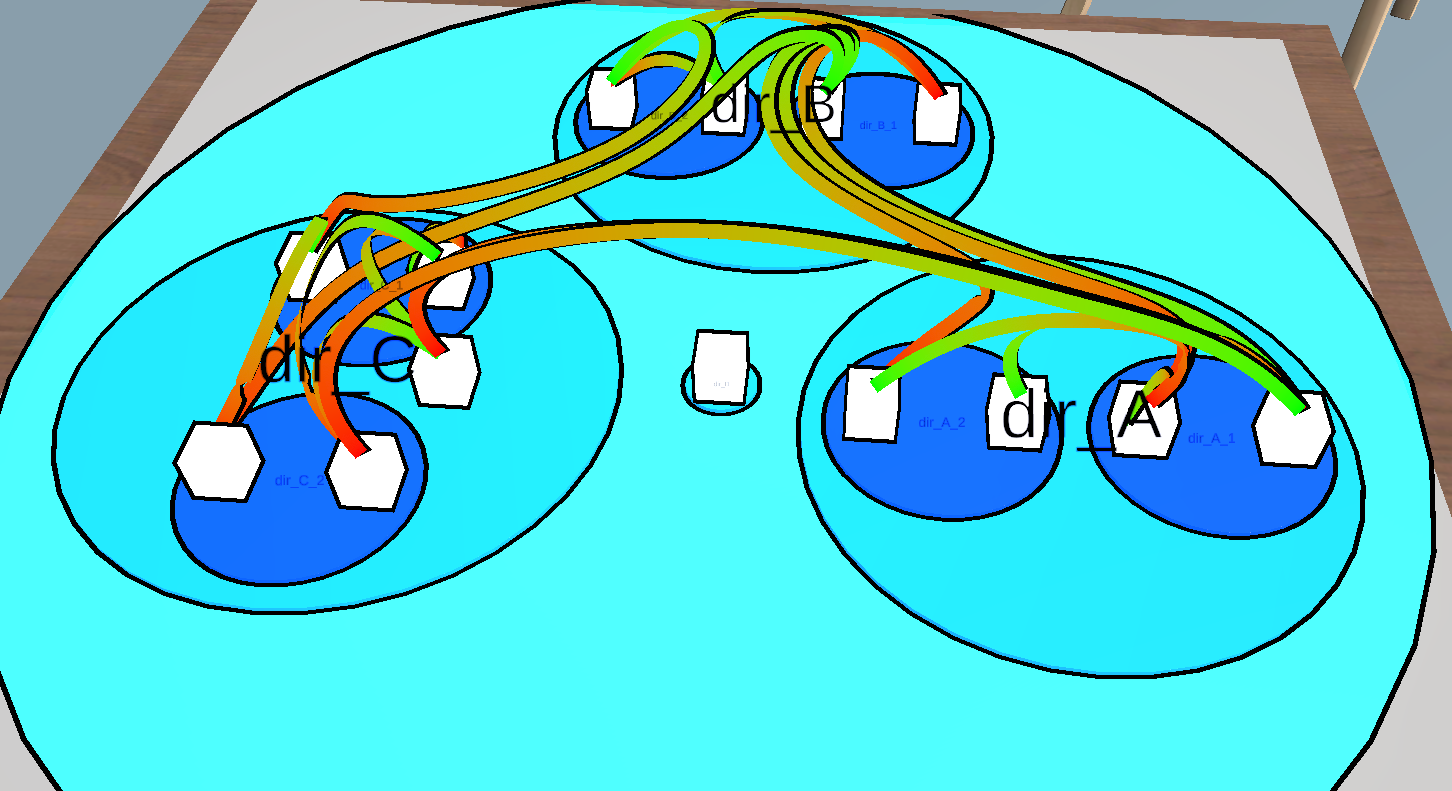
\includegraphics[width=1\textwidth]{Evaluation/img/city_1.png}
  \caption{The first \gls{city} for the user study}\label{fig:city1}
\end{figure}

\begin{figure}[H]
  \centering
  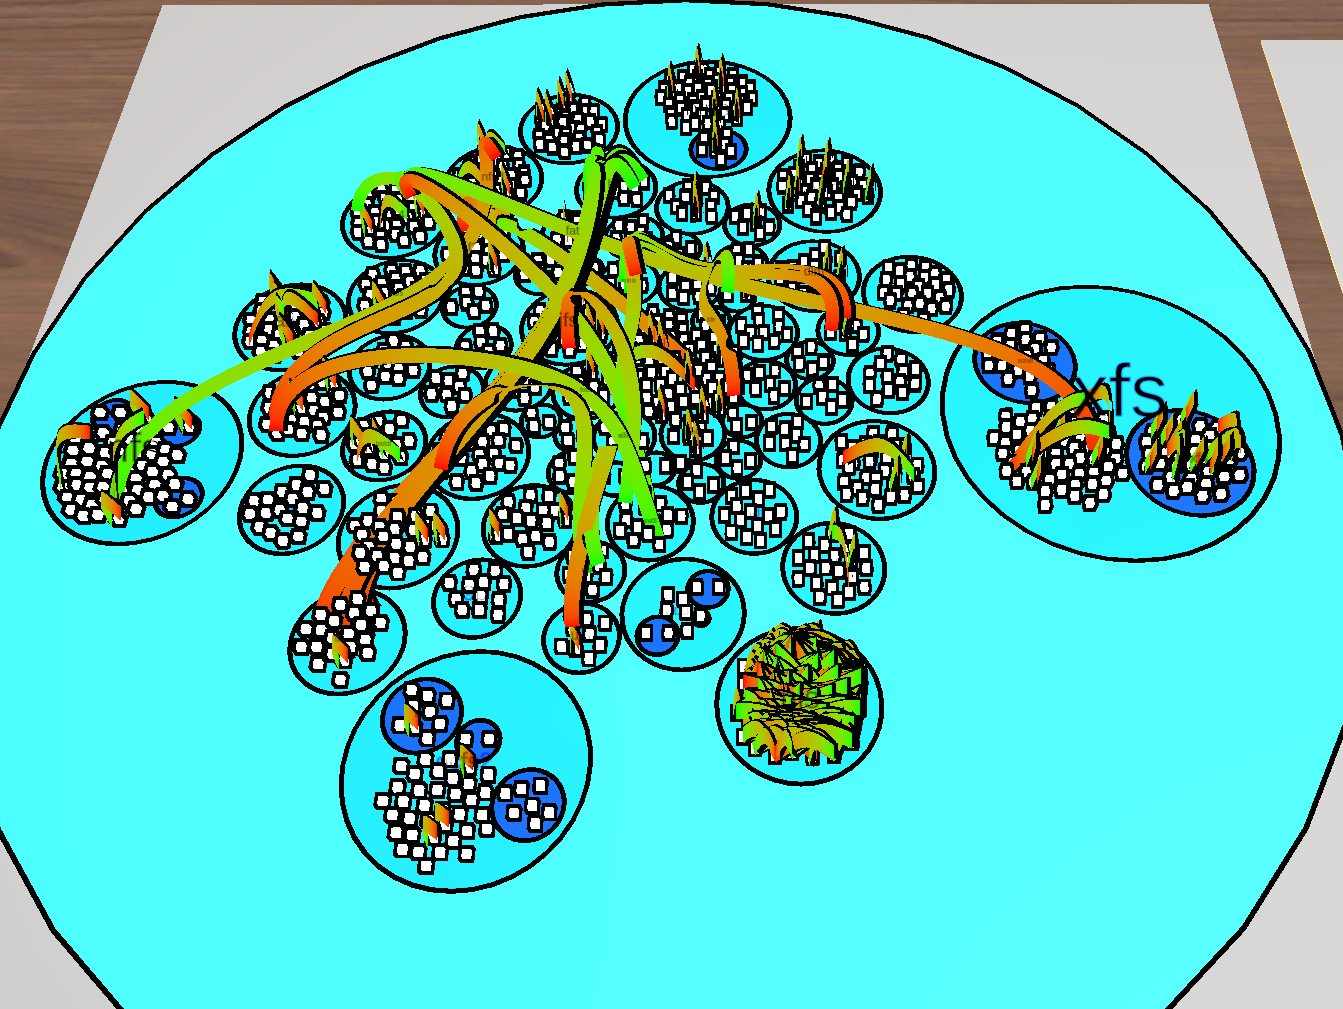
\includegraphics[width=1\textwidth]{Evaluation/img/city_2.png}
  \caption{The second \gls{city} for the user study}\label{fig:city2}
\end{figure}

\begin{figure}[htb]
  \centering
  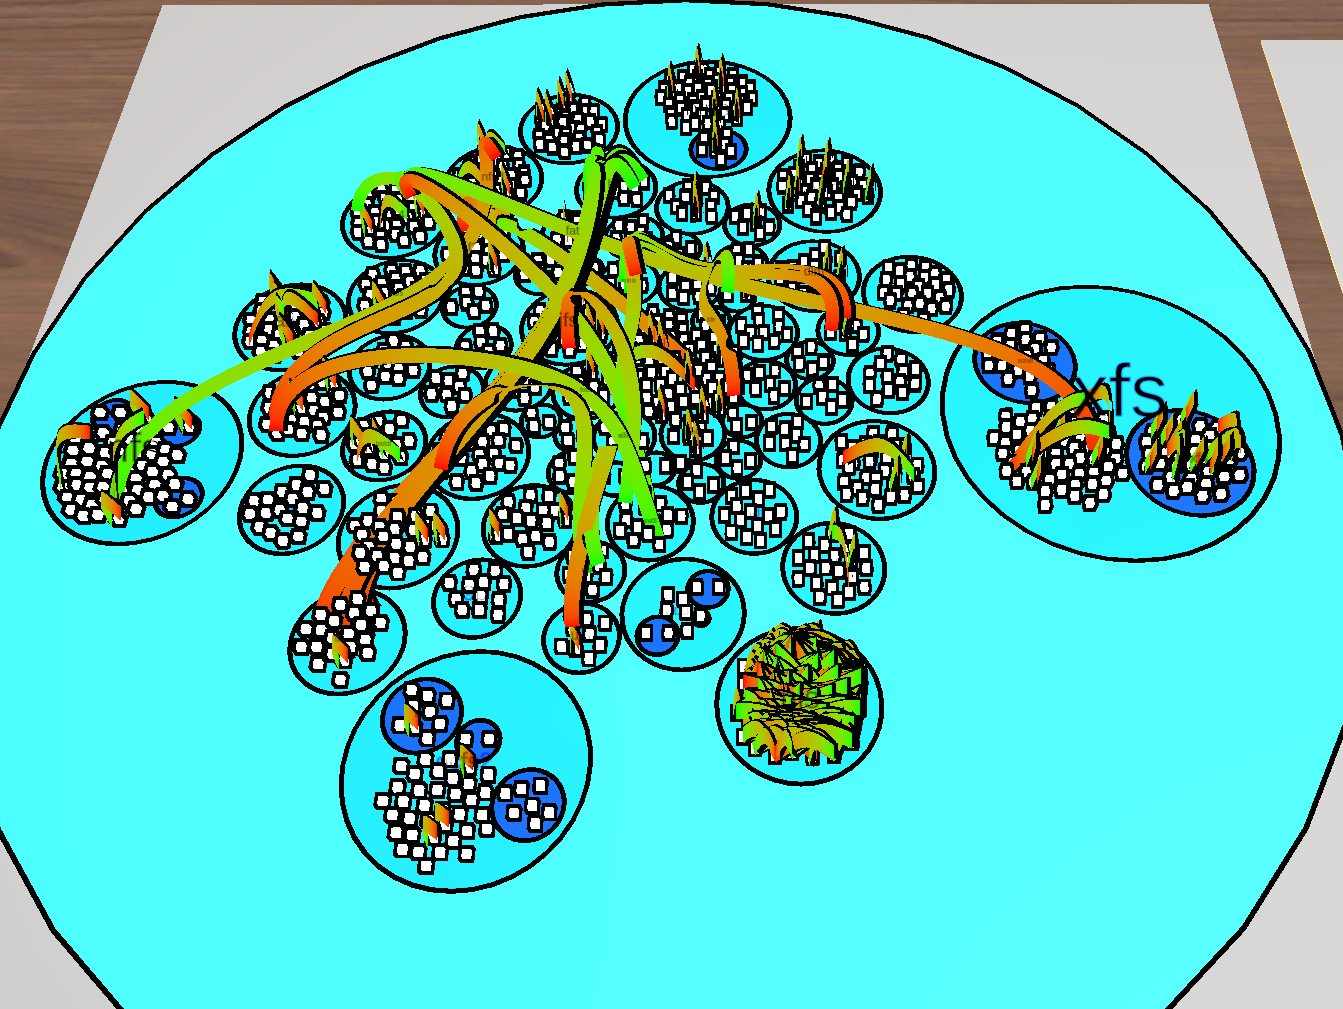
\includegraphics[width=1\textwidth]{Evaluation/img/city_3.png}
  \caption{The third \gls{city} for the user study}\label{fig:city3}
\end{figure}
In this survey the subjects will be asked various demographic questions as well as what Android device and version they will be using.
In addition to that the subjects will be asked if they are experienced with \gls{see} and if they are experienced with software development.
Before the subjects will be asked to solve various tasks they will be asked to watch a short tutorial video on each application.
After the video they will get a training task where every subject can get used to the system and ask questions if they have trouble solving the training task.
The overseer will also make sure that every essential action will be practiced such as zooming and moving the \gls{city}.
Figure \ref{fig:city1} shows a small arranged \gls{city} that shall be used for the training tasks.
The structure of the training \gls{city} is generic and follows a simple pattern.
That shall ensure that the user can focus on the training and that the user does not get overwhelmed.

Following the first questions and the training, the subjects can start with the main tasks.
For each application there will be two tasks and after each task the subjects will be handed a \gls{post-task} questionnaire.
Last but not least there will another questionnaire that aims to scale the \gls{usability} of the two applications.
For the \gls{post-task} questions the \gls{ASQ} will be used and for the \gls{usability} questions \gls{sus} will be used.
Both questionnaires will be discussed later on in section \ref{questionaires}.
For each main task the overseer will also take the completion time of every main task.
The first and second task on the first device will be performed on the \gls{city} that can be seen in figure \ref{fig:city2} and the third and forth task on device two will be performed on the \gls{city} that can be seen on figure \ref{fig:city3}.
These examples are much larger than the training \gls{city} and represent real life code.
The second \gls{city} shows the file system of Linux and the third one shows the network component of Linux.
That way the tasks might reflect better on real world uses for \gls{see}.

To not exhaust the testers too much the experiment shall not take longer than one hour.
This also ensures that there is no to little variance due to exhaustion.
Each participant might have a different concentration span, but this shall not be the focus of this experiment.

\subsection{Realization}
\label{real}
The following sections will cover the realization of the previously planned study. 
The choice of the used survey tool and questionnaires will be explained in section \ref{survey} and section \ref{questionaires}.
Afterwards a pilot study will be executed to test the study and possibly find missing aspects in section \ref{pilot}.
Finally, the final experiment set up will be discussed in section \ref{final}.

\subsubsection{Survey tool}
\label{survey}
As a survey tool Google Forms\footnote{https://www.google.com/forms/about/ (last visit: 05.06.2022)} will be used.
The survey tool has to fulfill the following requirements: 
\begin{itemize}
  \item The study will be online because an overseer has to attend every experiment, and therefore it comes in handy to be flexible in terms of location. For this reason the survey shall be fully in a browser. 
  \item The survey tool should be free to use.
  \item Subjects shall be anonymous.
  \item The results shall be exportable in a data format like \gls{csv}
  \item Subjects should have the option to presave their answers. In addition to that answers should not be lost on reload.
  \item There should be an option to embed the introduction videos in the survey.
\end{itemize}

Google Forms fulfills all these requirements and will therefore be used. 
The final form can be seen in figure \ref{fig:intro} which shows the intro of the survey and in figure \ref{fig:video} which shows the embedded intro video for \gls{see} mobile.
\begin{figure}[H]
  \centering
  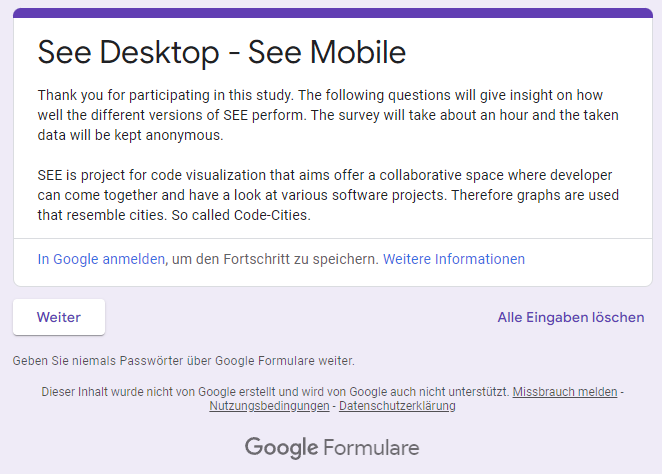
\includegraphics[width=1\textwidth]{Evaluation/img/form_intro.png}
  \caption{The intro of the survey}\label{fig:intro}
\end{figure}

\begin{figure}[H]
  \centering
  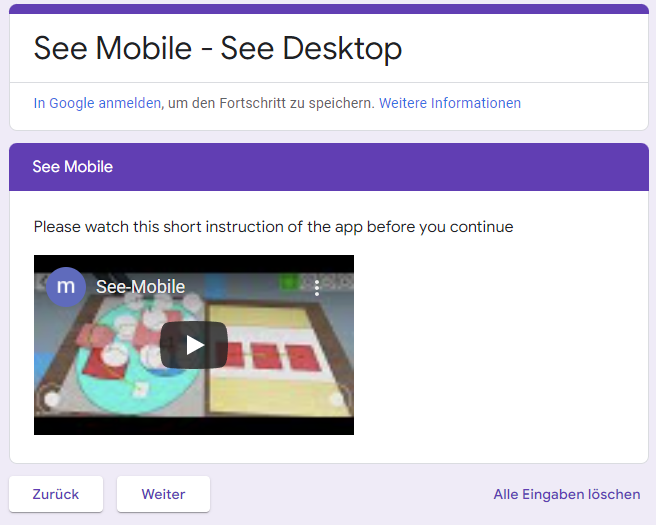
\includegraphics[width=1\textwidth]{Evaluation/img/form_video.png}
  \caption{The introduction video of the survey}\label{fig:video}
\end{figure}

\subsubsection{Questionnaires}
\label{questionaires}
There will be three questionnaires used for the study that will be discussed in detail in the following.
The study will start with a demographic questionnaire that covers general information about the subject.
After every task there will be \gls{ASQ} and after every block of tasks for each of the two covered devices there will be a \gls{sus} questionnaire.
\paragraph{Demographic questionnaire}\mbox{}\\
The subjects shall start the survey with a demographic questionnaire.
In that section they will be asked for their age, gender, the highest degree, experience with \gls{see}, experience with first person video games, their Android device name, their Android version and their experience with software development.
These specifications will be used to form different groups to see if there is any impact on the result of the following measurements. 
\cite{Mclellan2011} has shown that the user experience can have a significant impact on the \gls{sus}-score.
It is therefore important to view the measured results in context of the paired demographic data.

The mobile version was only tested on a single Android device.
It is likely that the performance of the application varies on different Android versions or devices.

\paragraph{Post-task questionnaire}\mbox{}\\
The \gls{post-task} questionnaire will supplement the \gls{post-study} questionnaire on a micro level.
The main focus here will be on single tasks, which allows to have a look at different aspects like effort, complexity and information provided by the system. 

As a \gls{post-task} questionnaire the \gls{ASQ} will be used. 
The \gls{ASQ} was first introduced in 1991 by \cite{lewis1991psychometric}.
It is designed for task based surveys and contains three questions.
The \gls{ASQ} will be used because it brings the following advantages:
\begin{itemize}
  \item The questionnaire has been used many times over the years and has proven its validly (\cite{hajesmaeel2022most}; \cite{lewis1991psychometric}; \cite{lewis1995ibm}).
  \item With its three questions it is short and does not exhaust the subjects. This is especially important because it will be required to finish this questionnaire a total of four times.
  \item It fits well for this study because it is a questionnaire designed for task based evaluations.
\end{itemize}
The \gls{ASQ} consists of three questions that scale from one to seven where one means \enquote{strongly disagree} and seven means \enquote{strongly agree}.

\paragraph{Post-study questionnaire}\mbox{}\\
The \gls{post-study} questionnaire is mainly to obtain as much information about the \gls{usability} of the two systems as possible.
The questionnaire can be longer than the \gls{post-task} but still should not be to long to keep the processing time of the survey at around an hour.

The \gls{sus} questionnaire was first published in 1986 by John Brooke (\cite{brooke1996sus}) and is therefore widely used and proven as citations in more than 1200 publications up until 2013 show (\cite{brooke2013}).
The \gls{sus} is used in this study for the following advantages: 
\begin{itemize}
  \item It consists of ten questions and has to be done two times. Twenty questions in total fit well into the planned one hour total time span of this experiment.
  \item It has been made publicly available and is free to use (\cite{brooke1996sus}).
  \item It is widely used and therefore already proven to give useful results (\cite{brooke2013}; \cite{lewis2018system}; \cite{grier2013system}).
  \item According to \cite{doi:10.1177/1541931213571043} and \cite{doi:10.1080/10447310802205776} it is suited to compare two systems.
  \item Besides \gls{usability} \cite{10.1007/978-3-642-02806-9_12} finds that also learnability is measured, which will also be looked at later on in section \ref{results}.
\end{itemize}
The \gls{sus} questionnaire will contain as already mentioned ten questions.
Each question will give a five-level rating from \enquote{strongly disagree} to \enquote{strongly agree}.
The results will then be combined into a \gls{usability}-score from zero to 100 where a high value represents a good result and a low value a bad one.
\subsubsection{Pilot study}
\label{pilot}
In a first test the pilot study was executed with one tester.
Afterwards the study was discussed and checked for errors.
It stood out that the example \gls{city} of task one was too different to the one in the second task.
Therefore, the \gls{city} of the first task was exchanged with a larger and better comparable one.
Further on a \gls{city} with 1288 nodes (see figure \ref{fig:city2}) as well as one with 1464 nodes (see figure \ref{fig:city3}) will be used.

Also, the tasks were not comparable because they differed in the types of interactions they used.
In one task the user was asked to rename a node and in the other one the user shall add four nodes.
For renaming a node the user has to use a keyboard which does not make it comparable to just click and add nodes in the second task.

\begin{figure}[htb]
  \centering
  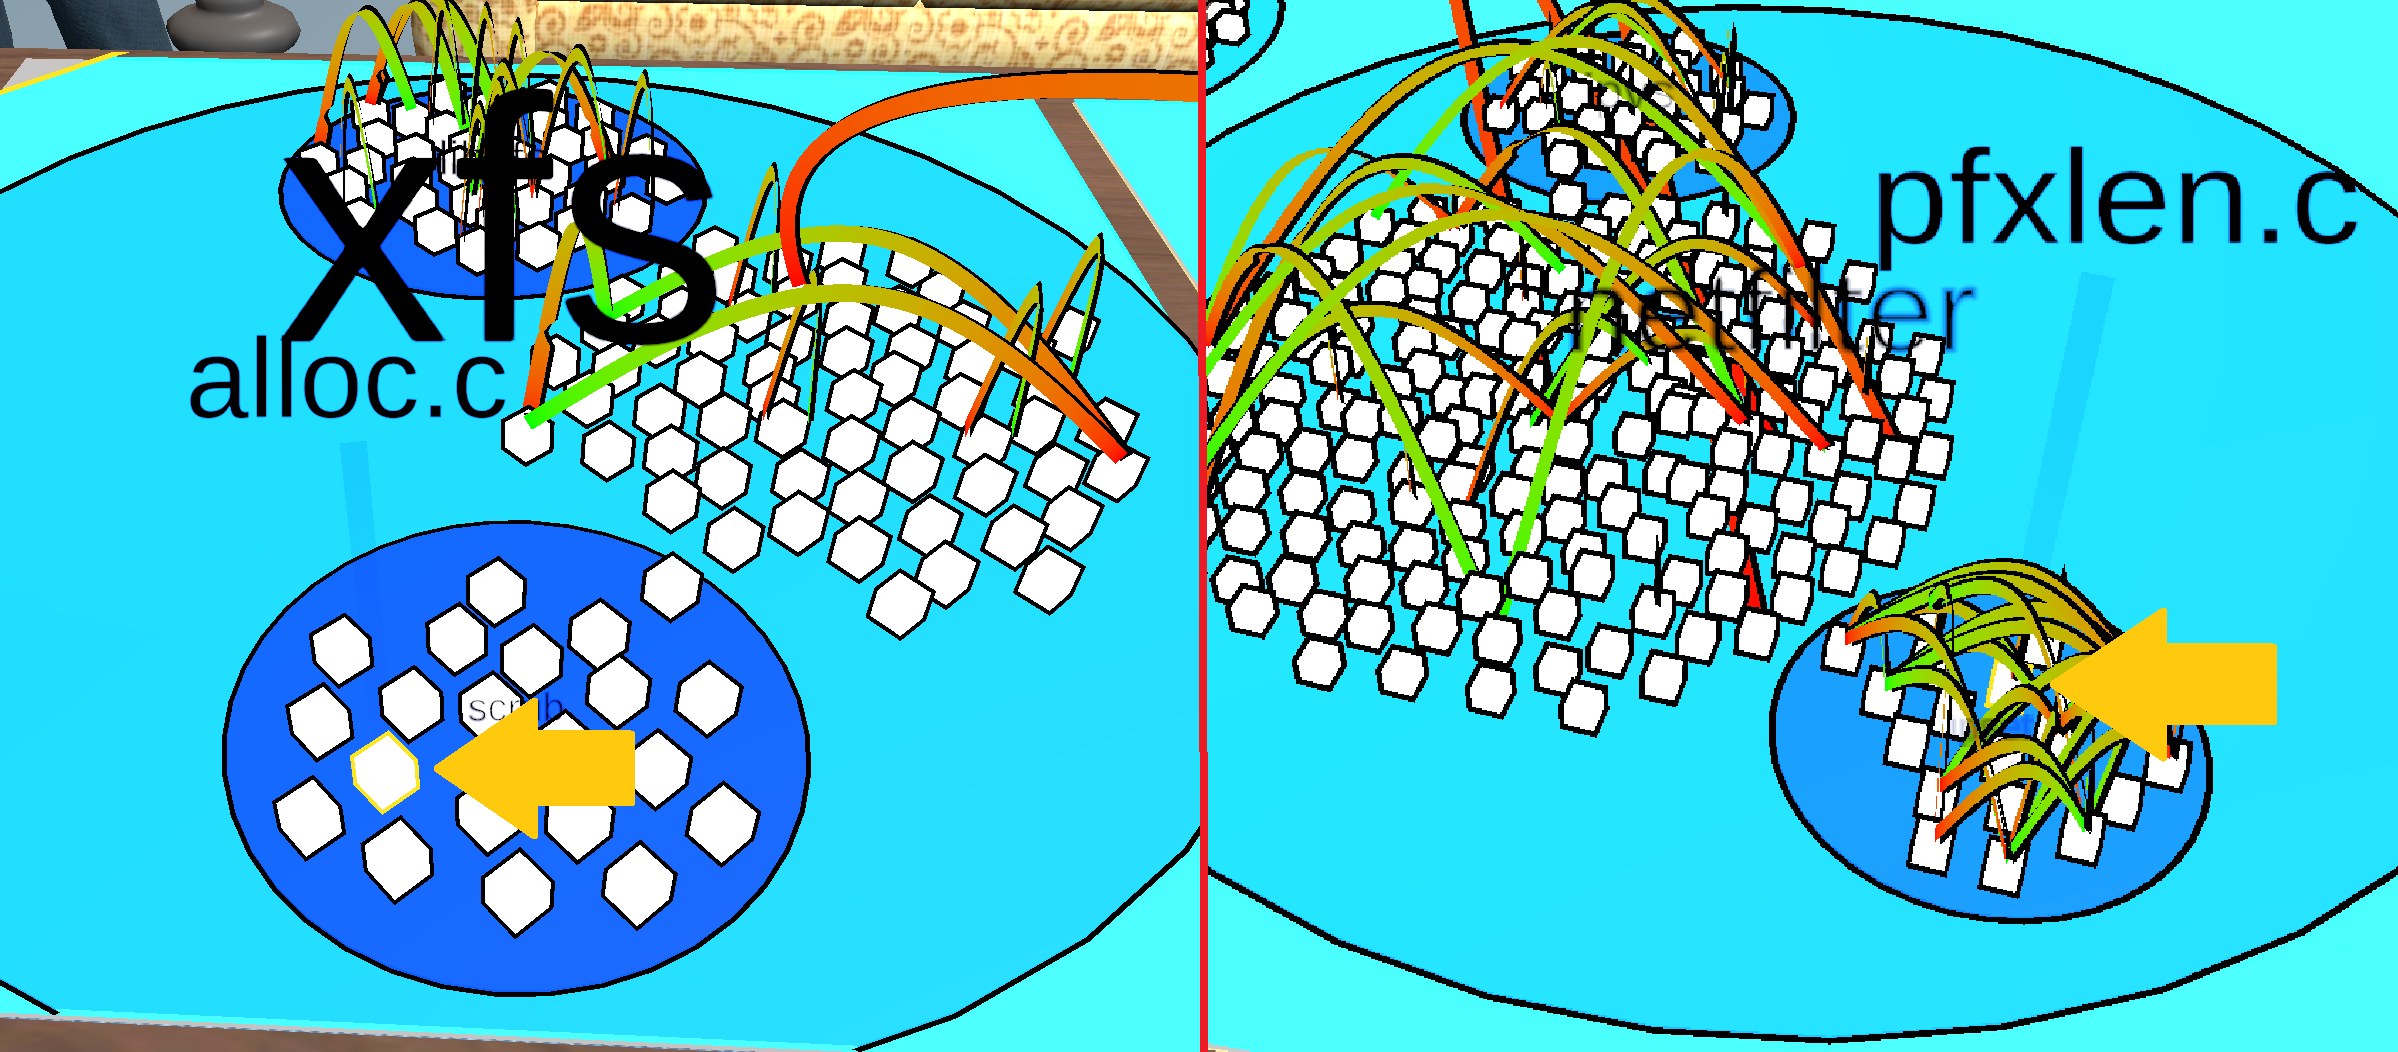
\includegraphics[width=1\textwidth]{Evaluation/img/task1.png}
  \caption{The two key nodes are marked with a yellow arrow}\label{fig:task1}
\end{figure}

\subsubsection{Final experiment set up}
\label{final}
Demographic questions:
\begin{itemize}
  \item Age
        \begin{itemize}
          \item 0-15 years old
          \item 16-30 years old
          \item 31-45 years old
          \item 46+ years old
        \end{itemize}
  \item What gender do you identify as?
        \begin{itemize}
          \item Male
          \item Female
          \item Other ...
          \item Prefer not to say
        \end{itemize}
  \item What is the highest degree or level of education you have completed?
        \begin{itemize}
          \item Some High School (Hauptschule/Realschule...)
          \item High School (Abitur)
          \item Bachelor's Degree
          \item Master's Degree
          \item Ph.D. or higher
          \item Prefer not to say
          \item Other ...
        \end{itemize}
\end{itemize}

Questions regarding used hardware and experience
\begin{itemize}
  \item Are you already experienced with See?
  \item Do or did you play first person video games?
  \item Do or did you develop software?
  \item On which Android device will you attend?
  \item Which Android version are you using?*
\end{itemize}

\begin{table}[]
  \resizebox{\textwidth}{!}{%
    \begin{tabular}{lll}
      Nr.                                                                                                                                                                                         &
      Task                                                                                                                                                                                        &
      Expected time                                                                                                                                                                                 \\ \hline
      Training                                                                                                                                                                                    &
      \begin{tabular}[c]{@{}l@{}}Navigate through the planes "dir\_root" \\ \textgreater "dir\_B" \textgreater "dir\_B\_2". On that plane \\ select "b2\_b.cpp" and rename it "b42".\end{tabular} &
      1 - 5 mins                                                                                                                                                                                    \\
      1                                                                                                                                                                                           &
      \begin{tabular}[c]{@{}l@{}}Detect the largest plane "xfs". On that\\ plane find plane "scrub". Then find \\ and delete node "alloc.c".\end{tabular}                                         &
      0.5 - 5 mins                                                                                                                                                                                  \\
      2                                                                                                                                                                                           &
      \begin{tabular}[c]{@{}l@{}}Find the plane with one blue child \\ plane ("btrfs"). On the blue child \\ plane "tests" add four new nodes.\end{tabular}                                       &
      1 - 5 mins                                                                                                                                                                                    \\ \hline
      Training                                                                                                                                                                                    &
      \begin{tabular}[c]{@{}l@{}}Navigate through the planes "dir\_root" \\ \textgreater "dir\_C" \textgreater "dir\_C\_2". On that plane \\ select "c2\_b.cpp" and rename it "c42".\end{tabular} &
      1 - 5 mins                                                                                                                                                                                    \\
      3                                                                                                                                                                                           &
      \begin{tabular}[c]{@{}l@{}}Detect the \\ largest plane "netfilter". On that plane\\ find plane "ipset". Then find and \\ delete node "pfxlen.c".\end{tabular}                               &
      0.5 - 5 mins                                                                                                                                                                                  \\
      4                                                                                                                                                                                           &
      \begin{tabular}[c]{@{}l@{}}On the plane with the most \\ edges ("ipv6") find the smallest plane\\ "ila" and connect all four nodes on it.\end{tabular}                                      &
      1 - 5 mins                                                                                                                                                                                    \\ \hline
    \end{tabular}%
  }
  \caption{The tasks used for the experiment. The device will be switched after task 2.}
  \label{table:tasks}
\end{table}

\begin{table}[]
  \resizebox{\textwidth}{!}{%
    \begin{tabular}{llll}
      Phase          &                        & \multicolumn{2}{l}{Description}                                          \\ \hline
      Pre-Experiment &                        & \multicolumn{2}{l}{Demographic questionnaire}                            \\ \hline
                     & City                   & Group 1                                       & Group 2                  \\ \hline
      Training       & Figure \ref{fig:city1} & \multirow{6}{*}{Desktop}                      & \multirow{6}{*}{Mobile}  \\
      Task 1         & Figure \ref{fig:city2} &                                               &                          \\
      ASQ            &                        &                                               &                          \\
      Task 2         & Figure \ref{fig:city2} &                                               &                          \\
      ASQ            &                        &                                               &                          \\
      SUS            &                        &                                               &                          \\ \hline
      Training       & Figure \ref{fig:city1} & \multirow{6}{*}{Mobile}                       & \multirow{6}{*}{Desktop} \\
      Task 3         & Figure \ref{fig:city3} &                                               &                          \\
      ASQ            &                        &                                               &                          \\
      Task 4         & Figure \ref{fig:city3} &                                               &                          \\
      ASQ            &                        &                                               &                          \\
      SUS            &                        &                                               &
    \end{tabular}%
  }
  \caption{Experimental procedure per subject. The procedure is swapped per group.}
  \label{table:procedure}
\end{table}


\subsubsection{Execution}
Before the study the subjects got an installation instruction as well as the two applications.
For the execution of the user study every subject got one of two links to a Google form.
Each form starts with a different device. 
The forms were handed out in alternating order and the subjects should therefore be assigned random to the two groups.

The study was executed within a week and a total of 20 subjects participated.
From the 20 subjects, two could not finish the tasks on their mobile device, which leaves n = 18 participants that finished the survey.

The overseer hosted an instance of \gls{see} from his home network and watched the subjects doing their task.
He also gave instructions for the training tasks and made sure that all essential interactions were trained such as zooming and moving the \gls{city}.
Every subject got the same training.


\subsection{Results}
The \hyperref[calc]{calc\_data.ipynb} script can be used to reproduce the result data for the following section.
Also, all shown diagrams in this section can be reproduced with the script.

In the following the group that started the study with the desktop version of \gls{see} will be called \textit{Group 1} and the group starting with the mobile version will be called \textit{Group 2}.
The task order of the two groups remains the same.
Both groups start with the same task.
That way not only both groups but also the desktop and the mobile \gls{see} version will be compared. 

In the coming up section the \gls{utest} will be used multiple times to see if there are significant differences between to data sets.
The \gls{utest} brings the advantage that the tested data sets do not need to fulfill the requirement of a normal distribution (\cite{gibbons1991comparisons}).
This is important because the sample size of n = 18 is too small to assume a normal distribution.
The used level of significance will be $\alpha = 0.05$.

\label{results}
\subsubsection{Demographic data}
In this subsection it will be verified if the two groups differ significantly in their demographic data. 
Therefore, a two-tailed \gls{utest} that checks whether a set of demographic values from \textit{Group 1} $\neq$  a set of demographic values from \textit{Group 2} will be used.
Both groups have a sample size of $n = m = 9 $ with $\alpha = 0.05$ which leads to a critical value of $U = 17$ for a two-tailed \gls{utest}.

\paragraph{Gender}\mbox{}\\
Of 18 participants, 17 reported being male. 
One participant preferred not to say his or her gender and can therefore not be grouped.
Due to this fact a grouping does not make sense here in general. 

\paragraph{Age}\mbox{}\\
The subjects were asked to choose their age in grouped options. 
Most of the participants were aged between 16 and 30 years.
Only two participants were aged between 31 and 45 years. 
Therefore, the age of the participants should not fall into account of the results of the study.

\paragraph{Highest degree}\mbox{}\\
Nine of the participants answered with \enquote{Bachelor's Degree} for their highest achieved degree. 
It is therefore the most common option as pictured in figure \ref{fig:degree}.

To measure the \gls{utest} the options were put into an ordinal scale which follows the same order as in the survey.
The test shows there is no significant difference between the two groups ($U = 33.0; p \approx 0.51$).

\begin{figure}[H]
  \centering
  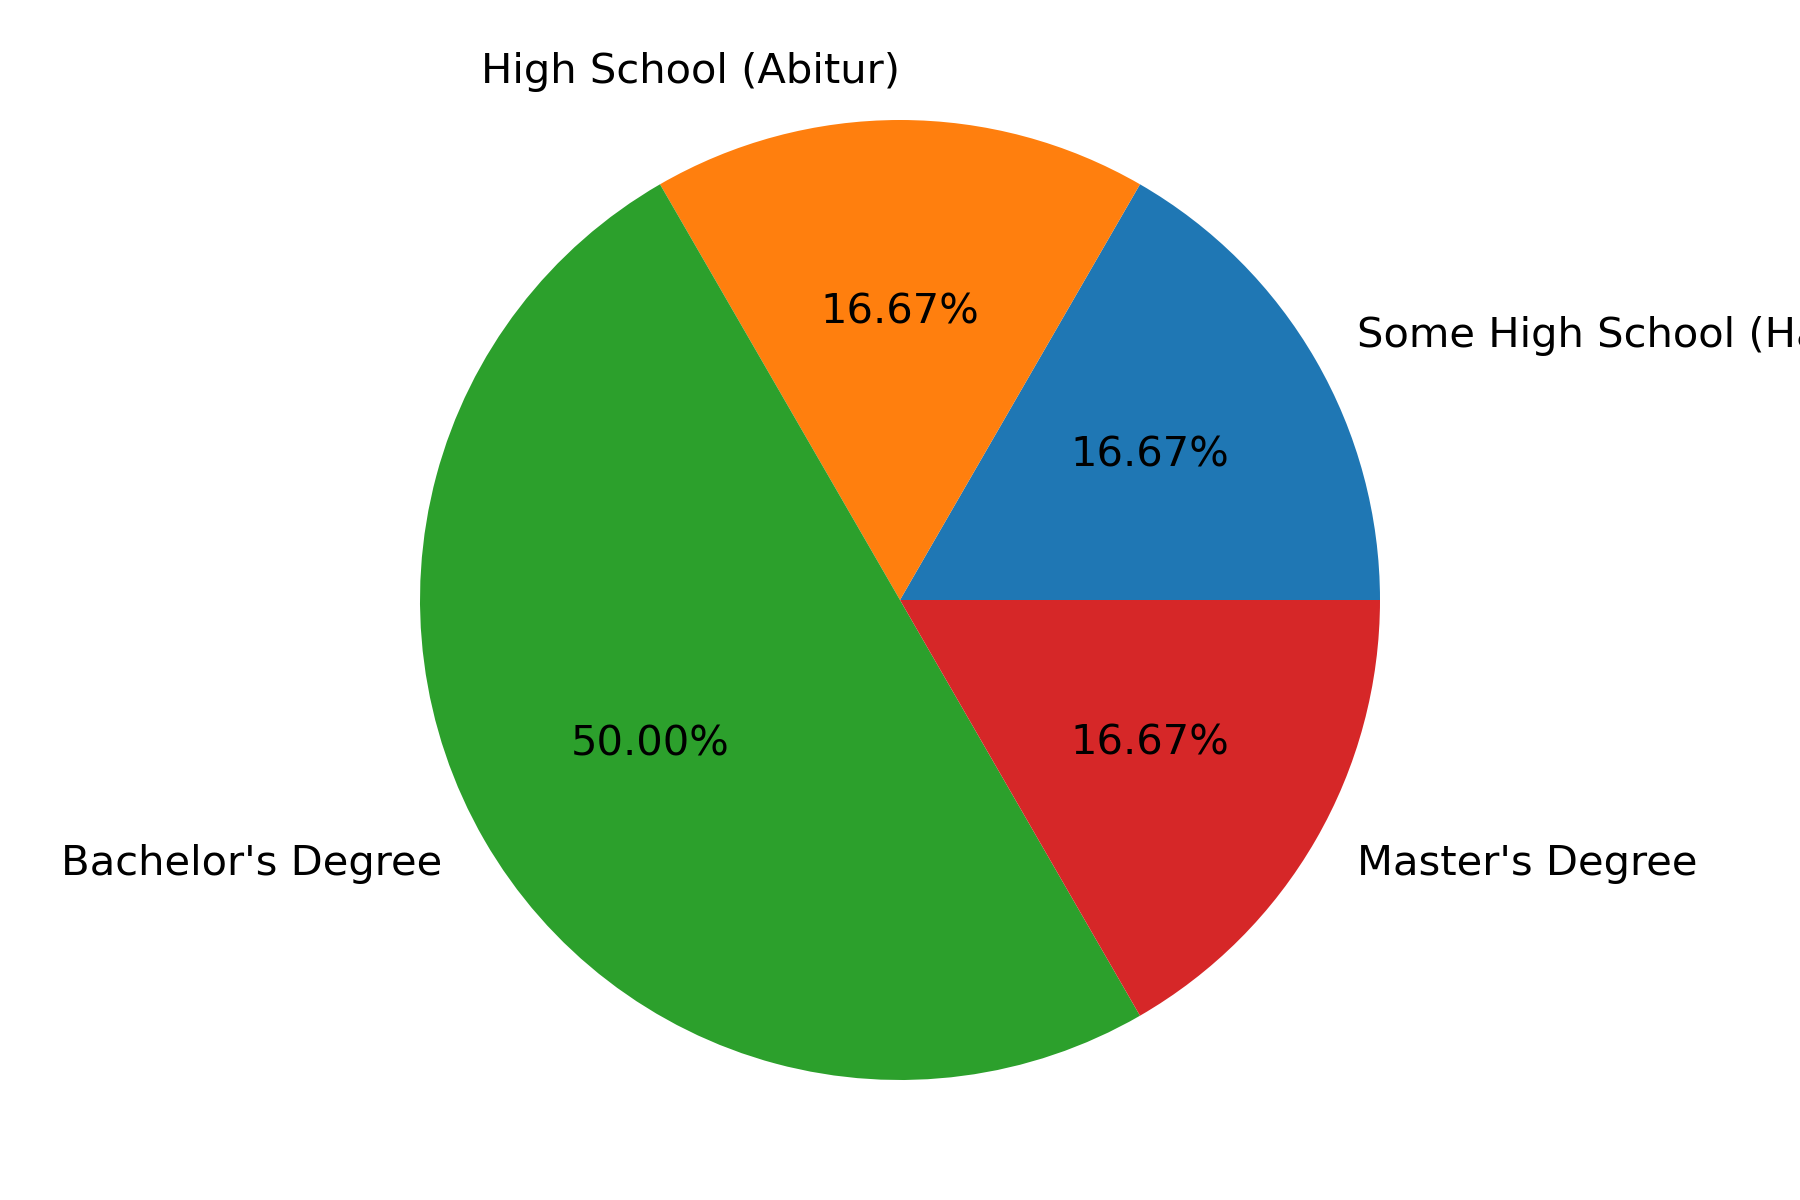
\includegraphics[width=0.7\textwidth]{Evaluation/img/degree.png}
  \caption{The distribution of the highest completed degrees of all 18 subjects}\label{fig:degree}
\end{figure}

\paragraph{Experience}\mbox{}\\
The subjects were asked if they had experience regarding \gls{see}, software development and first person video games.
All but one subject had experience with first person video games and the single subject without experience had at least experience with \gls{see} which could arguably count as a first person video game.
Therefore, experience with first person video games should not have an impact on this study.

Five of 19 subjects had experience with \gls{see}.
The \gls{utest} shows there is no significant difference between the two groups ($U = 27.0; p \approx 0.23$).
Even though there is no significant difference, four of the subjects with \gls{see} experience are in \textit{Group 2} and only one in \textit{Group 1}.

The majority of ten subjects had experience with software development.
The other eight subject had no experience.
The \gls{utest} shows there is no significant difference the two groups ($U = 49.5; p \approx 0.38$).

\paragraph{Android device and version}\mbox{}\\
A large variety of 17 different Android devices were used.
Therefore, the distribution of Android devices should not have impact on the study results.
Nonetheless, it has to be considered that the devices \enquote{Huawei P10 lite}, \enquote{Huawei P20 Pro} \enquote{Samsung A52S}, \enquote{Samsung S9} and the \enquote{Poco X3 Pro} had performance issues.
These performance issues showed in bumpy movement and player interactions.
Unfortunately, it could not be measured how strong the impact was on the performance on the single phones.
The threads of validity this could cause will be further discussed in section \ref{sec:validity}.
Three of the devices with bad performance belong to \textit{Group 1} and the other two to \textit{Group 2}.

The Android version was not distributed as much as the Android devices used. 
The most common used one was Android 12, which is also the most current one to the time of this writing.
Android 12 was used by seven subjects.
The second most used version was Android 11.
One subject used Android 7 on the \enquote{Huawei P10 lite}.
Which is remarkable because Android 7 was released in 2016\footnote{\url{https://android-developers.googleblog.com/2016/08/taking-final-wrapper-off-of-nougat.html} (10.06.2022, 12:37)} and the \enquote{Huawei P10 lite} was released a little later in March 2017\footnote{\url{https://www.gsmarena.com/huawei_p10_lite-8598.php} (10.06.2022, 12:37)} but \gls{see} still managed to work, if with lower performance.
The distribution of the used Android devices can be seen in \ref{fig:android_version}.
The \gls{utest} shows there is no significant difference the two groups ($U = 39.0; p \approx 0.93$).

\begin{figure}[htb]
  \centering
  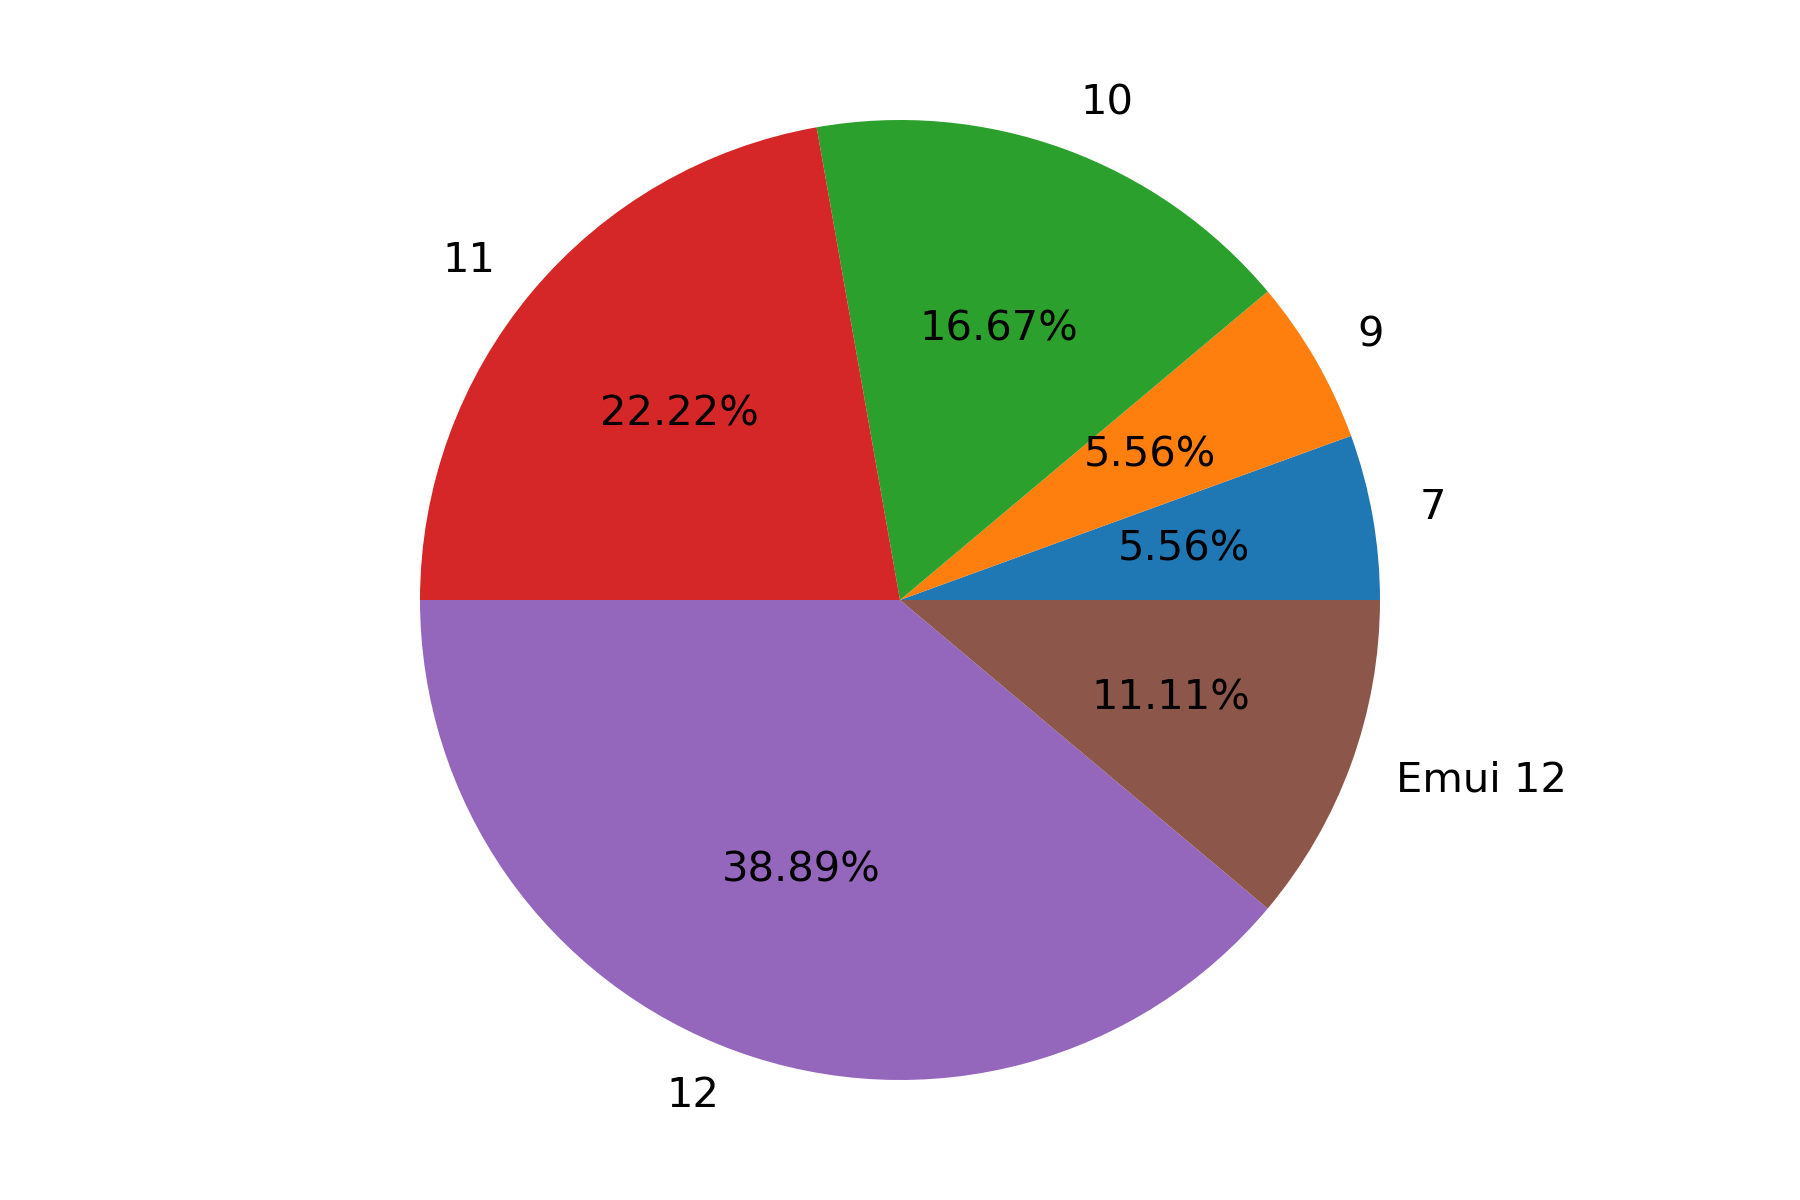
\includegraphics[width=0.7\textwidth]{Evaluation/img/droid_version.png}
  \caption{The distribution of the Android versions the subjects were using}\label{fig:android_version}
\end{figure}

\mbox{}\\
Surprisingly there has been no significant difference with the demographic data between the two groups.
In the following section the more exciting data will be analyzed. 

\subsubsection{Performance}
For the performance the time needed for each task was measured.
The time for the trainings task, however, was not measure because it would not fit the purpose of a training to be measured by time.
Therefore, the overseer asked the subjects to tell him when they begin the task. 
The time was taken after the subject has read and understood the task, and it was stopped when the subject successfully finished.
This will help to prove or discard hypothesis $H_{a}$.

Let's have a look at the two groups in general.
Is there any significant difference?
The total time needed for all subjects in the two groups can be seen in figure \ref{fig:group_time_violin}.
The average time \textit{Group 1} needed to complete all tasks was $\overline{t_1} = 487s$ and for \textit{Group 2} it was $\overline{t_2} = \approx388s$.
The median time for \textit{Group 1} was $\widetilde{t1} = 315s$ and for \textit{Group 2} it was $\widetilde{t_2} = 384s$.
As figure \ref{fig:group_time_violin} and the values mentioned above suggest the \gls{utest} shows there is no significant difference between the two groups with a $U = 43.0$ and $p \approx 0.86$.

\begin{figure}[htb]
  \centering
  \includegraphics*[width=1\textwidth]{Evaluation/img/group_time_violin.png}
  \caption{Total time each group needed as violin plot}
  \label{fig:group_time_violin}
\end{figure}

Furthermore, let's look at the single tasks. 
Has there maybe been a learning effect or difference in general between the groups? 
To find out task 1 from \textit{Group 1} will be compared with task 3 from \textit{Group 2} and so on.
Every couple of tasks is comparable because they have been done on the same device and use the same set of user interactions as described in section \ref{final}.
The \gls{utest} shows that there is no significant difference in any combination as listed below:
\begin{itemize}
  \item \textit{Group 1}, task 1 \& \textit{Group 2}, task 3: $U = 26.5; p \approx 0.23$
  \item \textit{Group 1}, task 2 \& \textit{Group 2}, task 4: $U = 35.5; p \approx 0.69$
  \item \textit{Group 1}, task 3 \& \textit{Group 2}, task 1: $U = 49.0; p \approx 0.48$
  \item \textit{Group 1}, task 4 \& \textit{Group 2}, task 2: $U = 57.0; p \approx 0.16$
\end{itemize}

Finally, let's see if there is a significant difference between the two used versions of \gls{see} in the single tasks.
The time needed for every single task on both versions can be seen in figure \ref{fig:speed_violin}.
There are some results that stand out and took way longer than the medians would suggest.
That could be caused by various reasons as for example:
\begin{itemize}
  \item The mobile version of \gls{see} did not run smooth on the subjects device and therefore the tasks became harder.
  \item The subject did not understand the task correctly and has to reread it.
  \item The subject overlooked a key object and continued the search at wrong areas.
\end{itemize}


\begin{sidewaysfigure}
  \centering
  \includegraphics*[width=1.15\textwidth]{Evaluation/img/speed1_violin.png}
  \caption{Violin plots of all tasks by device}
  \label{fig:speed_violin}
\end{sidewaysfigure}

\subsubsection{Usability}
\paragraph{ASQ}\mbox{}\\
...
\paragraph{SUS}\mbox{}\\
\begin{table}[htb]
  \resizebox{\textwidth}{!}{%
  \begin{tabular}{l|l|l|l|l|l|l|l|l|l|l|l|l|l|l|l|l|l|l}
  D & 60 & 58 & 80 & 60 & 78 & 70 & 85 & 53 & 80 & 88 & 80 & 50 & 63 & 85 & 50 & 93 & 100  & 85 \\
  M & 38 & 53 & 83 & 53 & 53 & 30 & 88 & 35 & 43 & 86 & 48 & 48 & 55 & 90 & 50 & 88 & 98 & 58
  \end{tabular}%
  }
  \caption{The \gls{sus}-scores from all 18 subjects. The first row contains the \gls{sus}-scores for the desktop application and the second row for the mobile application. The figures have been rounded to whole numbers.}
  \end{table}

  \begin{figure}[H]
    \centering
    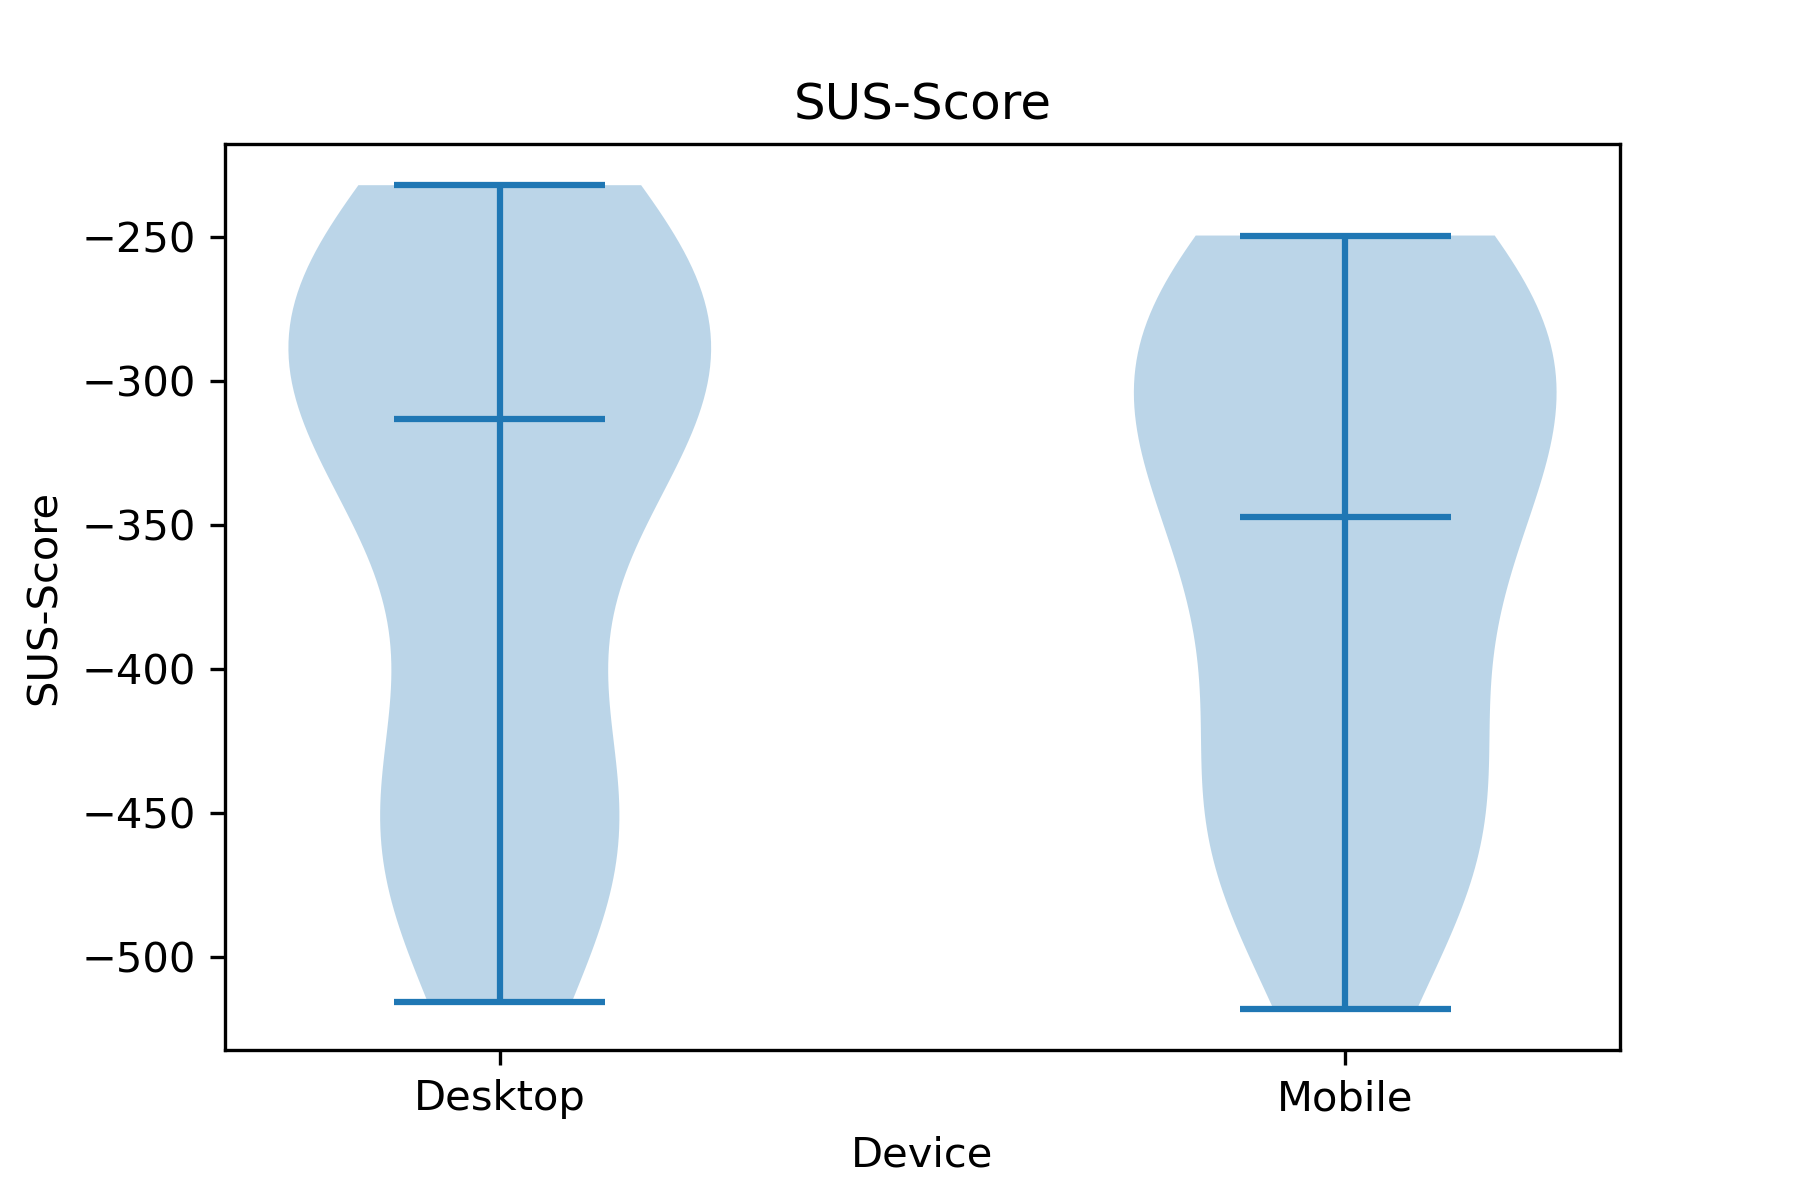
\includegraphics[width=1\textwidth]{Evaluation/img/SUS-Score_violin.png}
    \caption{The SUS-Scores of the two \gls{see} versions}\label{fig:sus-vio}
  \end{figure}

  \subsection{Threads to validity}
  \label{sec:validity}